\section{PROPENSITY SCORE MATCHING IN ACCOUNTING RESEARCH}

\paragraph{会計研究における PSM の利用 (Table 1 Panel A)}

\begin{table}
 \centering
 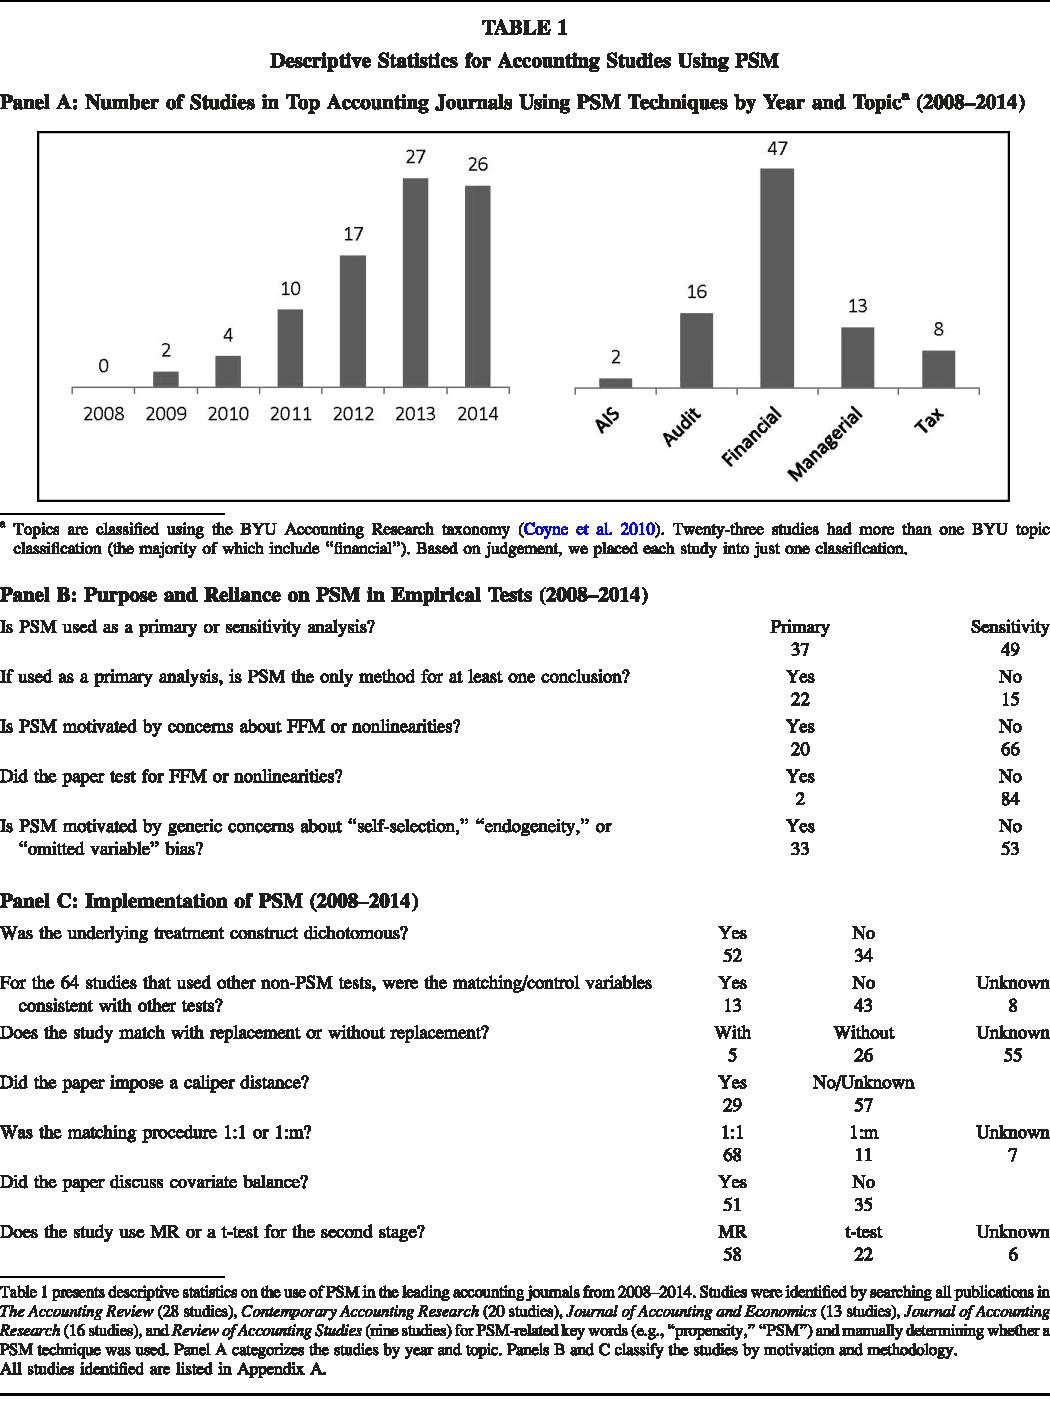
\includegraphics[width=14cm]{../table/tbl01.pdf}
\end{table}

\begin{itemize}
 \item 2008 $\sim$ 2014 年における、\textit{The Accounting Review,
       Contemporary Accounting Research, Journal of Accounting and
       Economics, Journal of Accounting Research, and Review of
       Accounting Studies} に掲載された論文延べ 86 件が対象。
 \item 会計研究で PSM が用いられはじめたのは最近 (86 件中 70 件は 2012
       $\sim$ 2014 の期間に刊行)。
\end{itemize}

\paragraph{各研究の PSM の位置付け (Table 1 Panel B)}

\begin{itemize}
 \item 主要な分析 (primary analyses) として用いている研究が 37 件である
       のに対し、ロバスト・チェック (sensitivity or robustness tests) と
       して用いている研究は 49 件。
 \item PSM を採用する理由として FFM や重回帰分析の線形性の仮定を挙げてい
       る研究はわずか 20 件。
 \item PSM が対処しうる内生性の問題を提示することなく、広く ``自己選択
       (self--selection),'' ``内生性 (endogeneity),'' および ``欠落変数
       バイアス (omitted variable bias)'' への対応として PSM を用いてい
       る研究が 33 件ある。
 \item Heckman (1979) の代わりとして誤用してしまっている研究も存在する。
\end{itemize}

\paragraph{処置群の選択の方法 (Table 1 Panel C)}

\begin{itemize}
 \item 問題の所在
       \begin{itemize}
        \item 処置が 2 値変数 (dichotomous) であるならば、PSM の実施は単純である。
        \item しかしながら、多様な状況でマッチングを実施するため、連続 (あるい
              は順序) 変数に閾値を設けて変換することがある\footnote{2 値
              変数を用いた処置群の選択について、例えば修正再表示のアナウ
              ンスメントや IFRS のアドプションがあげられる。一方で、非 2
              値変数を用いた処置群の選択について、企業の所有構造や監査人
              の産業特殊性 (auditor industry specialization) があげられ
              る}。
       \end{itemize}
 \item 問題点
       \begin{itemize}
        \item このような場合、閾値の近傍の観測値が over--represent される
              傾向があり、それによって、効果の大きさ (および平均処置効果)
              が消失し、第 II 種の過誤が生じる可能性が増大する。
       \end{itemize}
 \item 連続変数を用いている研究の数
       \begin{itemize}
        \item 34 件。また、この影響により、効果の大きさのみならずサンプ
              ル・サイズも低下する。
        \item 59 (12) 件の研究において、MR のサンプル・サイズの大きさは
              PSM の 3 (10) 倍である。
        \item サンプルサイズが小さいほど、サブサンプルは母集団を代表しな
              くなる。
       \end{itemize}
\end{itemize}

\paragraph{コントロール変数の選択 (Table 1 Panel C)}

\begin{itemize}
 \item MR と PSM のいずれを用いるにせよ、同様のコントロール変数を用いる
       べきであるにもかかわらず、しばしば異なるコントロール変数が用いら
       れていることがわかった。
 \item MR からマッチングに用いた変数を除外することは、その変数が処置変数
       (treatment) にも結果変数 (outcome) にも影響を与えないこと、
       ひいては、その変数によるマッチングが不必要であることを意味するに
       他ならない。
 \item 分析においては、\textit{post hoc} なモデルの特定 (model
       specification) をおこなっているという疑念 (appearance; 外観) を避
       けるため、PSM と他のテストとの説明変数の不一致を検討すべきである。
\end{itemize}

\paragraph{傾向スコア推定後のマッチング・プロシージャ (Table 1 Panel C)}

\begin{itemize}
 \item 置換処理 (replace)
       \begin{itemize}
        \item 55 件の研究において、マッチングに際して置換処理がおこなわ
              れているか否か (matching is performed with or without
              replacement) 開示されていない。
        \item 開示している 31 件の研究のうち、5 件が置換あり、26 件が置
              換なしであった。
       \end{itemize}
 \item キャリパー距離 (caliper distance)
       \begin{itemize}
        \item マッチング・プロシージャとしてキャリパー距離を開示して
              いる研究は 29 件のみ。
        \item 開示されているキャリパー距離の分布は、0.00005 から
              0.23 までで、よく用いられている距離は 0.01 (4 件)、0.03 (6
              件)、および 0.10 (5 件) である。
       \end{itemize}
 \item 1 対 1 と 1 対多のどちらのマッチングを用いるか
       \begin{itemize}
        \item 1 対 1 (one--to--one) が 68 instances であるのに対し、1 対
              多 (one--to--many) が 11 instances である。
       \end{itemize}
\end{itemize}

\paragraph{covariate balance (Table 1 Panel C)}

\begin{itemize}
 \item マッチング変数の数 (number of matching variables)、キャリパー距離
       (caliper distance)、グループ・サイズ (group size) などの要因は、
       PSM によってサンプルに covariate balance が生じる程度に影響する。
 \item しかしながら、covariate balance の決定はマッチング・クオリティ
       についての主観的な判断を要求するため、マッチングが実際に適切な
       (sufficient) balance を達成しているか否か、しばしば不透明である。
 \item サーベイの結果、35 件はマッチされたサンプル (matched sample) の
       covariate balance について議論しておらず、4 件のみ傾向スコ
       アの平均差について議論している。
 \item 研究においては、残存した covariate imbalance の効果を緩和するため
       に、PSM のサブサンプルにおいて MR を使うことができる。
 \item サーベイの結果、58 件は (第 2 段階の) ATE を推定する際に MR を用
       いている、22 件は結果変数の距離を t 検定することによって、処置効
       果を推定している、そして、6 件は推定手法を開示していないというこ
       とが明らかとなった。
\end{itemize}

\paragraph{サーベイの結論}

\begin{itemize}
 \item 本節で指摘した問題点は現在の文献でも改善されていない。
 \item Heckman (1979) モデルについて含意を示した Lennox et al. (2012,
       589) の結論と同様に、われわれは、多数の研究が ``重要な計量経済学
       上の問題点および PSM の利用をとりまく問題点に対する理解
       (appreciation) がほとんど無いままに、'' PSM を実施していると結論
       付ける。 
\end{itemize}